\let\negmedspace\undefined
\let\negthickspace\undefined
%\RequirePackage{amsmath}
\documentclass[journal,12pt,twocolumn]{IEEEtran}
 \usepackage[utf8]{inputenc}
 \usepackage{graphicx}
 \usepackage{amsmath}
 \usepackage{mathrsfs}
\usepackage{txfonts}
\usepackage{stfloats}
\usepackage{bm}
\usepackage{cite}
\usepackage{cases}
\usepackage{subfig}
 \usepackage{amsfonts}
 \usepackage{amssymb}
 \usepackage{enumitem}
\usepackage{mathtools}
\usepackage{tikz}
\usepackage{circuitikz}
\usepackage{verbatim}
\usepackage[breaklinks=false,hidelinks]{hyperref}
\usepackage{listings}
\usepackage{calc}
\usepackage{float}
\usepackage{longtable}
\usepackage{multirow}
\usepackage{multicol}
\usepackage{color}
\usepackage{array}
\usepackage{hhline}
\usepackage{ifthen}
\usepackage{chngcntr}

\newcommand{\BEQA}{\begin{eqnarray}}
\newcommand{\EEQA}{\end{eqnarray}}
\newcommand{\define}{\stackrel{\triangle}{=}}
\bibliographystyle{IEEEtran}
%\bibliographystyle{ieeetr}
\def\inputGnumericTable{}
\let\vec\mathbf
\providecommand{\pr}[1]{\ensuremath{\Pr\left(#1\right)}}
\providecommand{\cdf}[2]{\ensuremath{F_{#1}\left(#2\right)}}
\providecommand{\sbrak}[1]{\ensuremath{{}\left[#1\right]}}
\providecommand{\lsbrak}[1]{\ensuremath{{}\left[#1\right.}}
\providecommand{\rsbrak}[1]{\ensuremath{{}\left.#1\right]}}
\providecommand{\brak}[1]{\ensuremath{\left(#1\right)}}
\providecommand{\lbrak}[1]{\ensuremath{\left(#1\right.}}
\providecommand{\rbrak}[1]{\ensuremath{\left.#1\right)}}
\providecommand{\cbrak}[1]{\ensuremath{\left\{#1\right\}}}
\providecommand{\lcbrak}[1]{\ensuremath{\left\{#1\right.}}
\providecommand{\rcbrak}[1]{\ensuremath{\left.#1\right\}}}
%\providecommand{\abs}[1]{\left\vert#1\right\vert}
\providecommand{\res}[1]{\Res\displaylimits_{#1}}
\newcommand{\myvec}[1]{\ensuremath{\begin{pmatrix}#1\end{pmatrix}}}
\newcommand{\mydet}[1]{\ensuremath{\begin{vmatrix}#1\end{vmatrix}}}
\newcommand{\PROBLEM}{\noindent \textbf{PROBLEM: }}
\newcommand{\solution}{\noindent \textbf{Solution: }}
\newcommand{\note}{\noindent \textbf{Note: }}
\newcommand{\tofind}{\noindent \textbf{To find: }}
\title{Assignment 1}
\author{srijan shahi\\BT21BTECH11007}
\date{}
\begin{document}
% make the title area
\maketitle
\begin{abstract}
	This document contains the solution for Assignment 1 (	ICSC Class 10 2017 Q.11(b))
\end{abstract}

\PROBLEM $ PQR $ is a triangle.$  S $ is a point on the side $ QR $ of $ PQR $ such that $\angle{PSR} = \angle{QPR}$.\\
Given $  QP = 8 cm$,$  PR = 6 cm $ and $ SR = 3 cm $\\
\begin{enumerate}
	\item  Prove $\Delta{PQR}$ $\sim$ $\Delta{SPR}$\\
	\item Find the length of sides $  QR $ and $ PS $\\
	\item $\dfrac{\text{area}(\Delta{PQR})}{\text{area} (\Delta{SPR})}$
\end{enumerate}

\solution

\begin{enumerate}
	\item In $ {\Delta}  $PQR and $ {\Delta} $SPR\\
	$\angle{PSR}$ = $\angle{QPR}$.\\
	$\angle{r}$ is common to both\\
	3rd angles are equal\\
	therefore $\Delta{PQR}$ $\sim$ $\Delta{SPR}$\\
	Hence sides are proportional.\\
	
	\item $\dfrac{QR}{PR} =\dfrac{PQ}{PS}=\dfrac{PR}{SR}$\\
	
	$\implies \dfrac{QR}{6}=\dfrac{8}{PS}=\dfrac{6}{3}$\\
	
	$ \implies QR=12  $  and $ PS = 4 $\\
	
	\item $\dfrac{\text{area}(\Delta{PQR})}{\text{area} (\Delta{SPR})} = \dfrac{6^2}{3^2}=\dfrac{4}{1}$
	
	
\end{enumerate}

\begin{figure}[!ht]
\centering
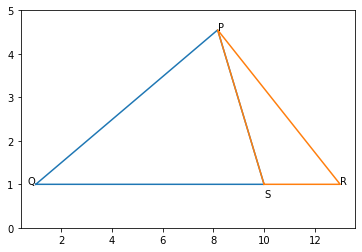
\includegraphics[width=\columnwidth]{download.png}
\caption{given similar triangle. 
Code: \texttt{codes/assign{\_}.py}}
\label{fig:triangle}
\end{figure}

\end{document}
